\section{Methodology}
\label{sec:data}

\vspace{-.3in}
\begin{figure}[h]
\centering
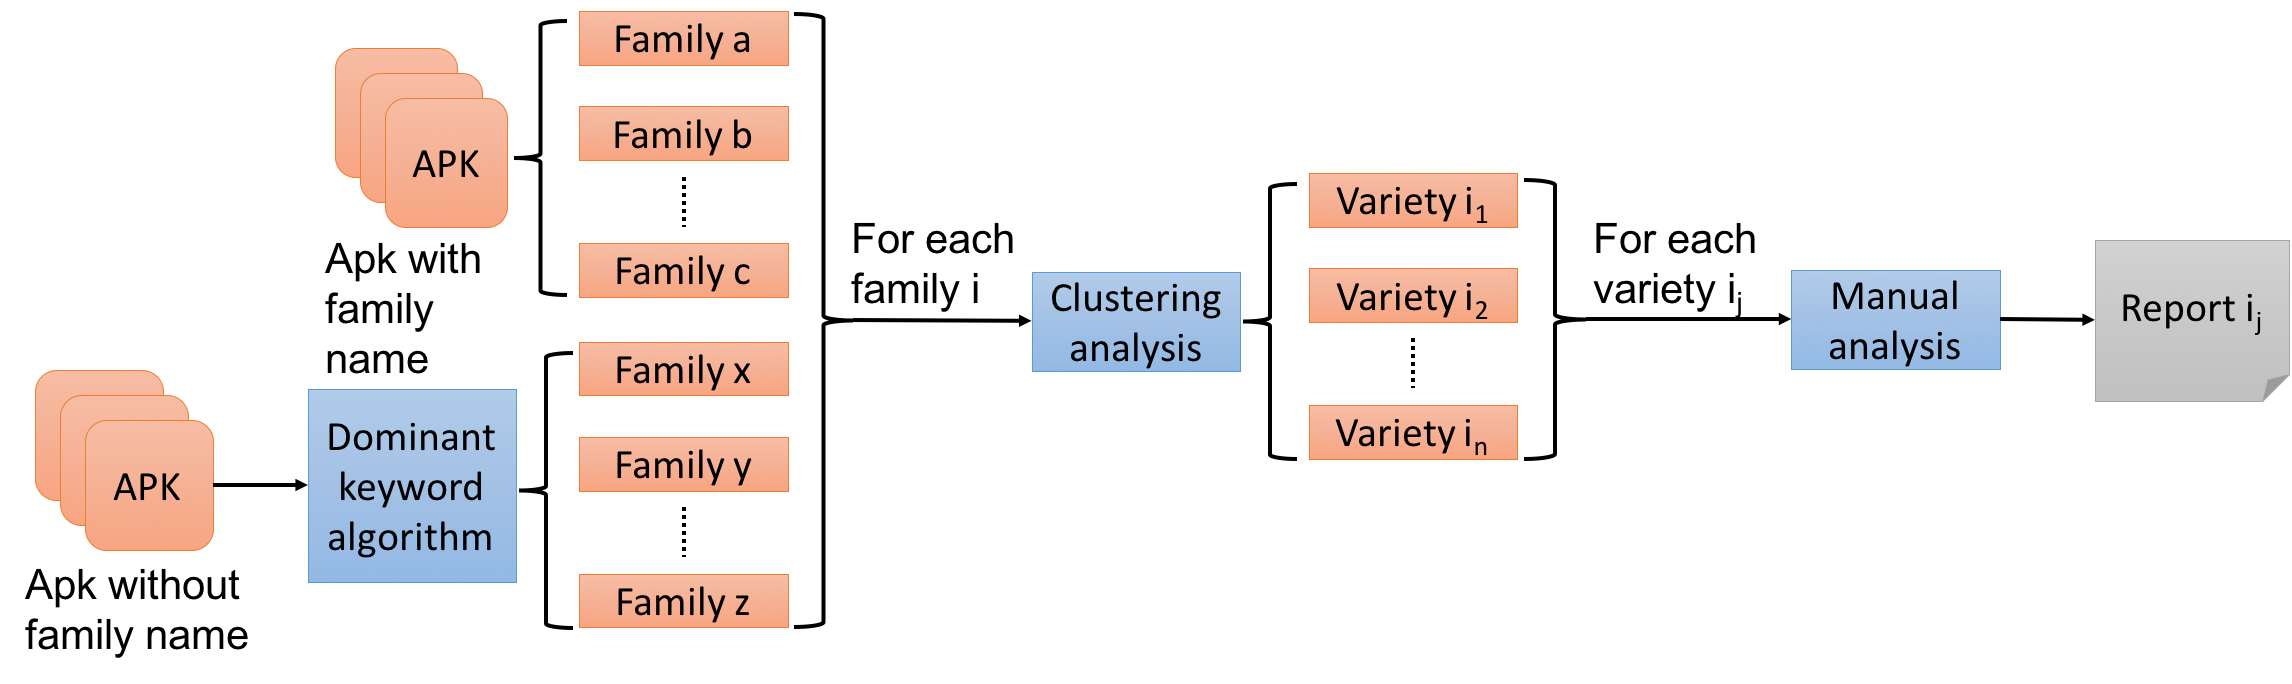
\includegraphics[width=4.5in]{fig/method-pipe.png}
\caption{Methodology pipeline: 
After malware families are identified, each family is categorized into semantically different varieties.
For each variety we generate a malware behavior report,
which is available at our \amd.}
\label{fig:methodpipe}
\end{figure}

We collect Android malware apps from multiple sources, analyze the samples, and report their detailed
behaviors.
Figure~\ref{fig:methodpipe} illustrates the pipeline of the methodology, which consists of
a two-step grouping process
followed by a manual procedure:
(a) Group malware samples with the same family name, 
(b) Categorize each family into semantically different varieties using a customized clustering analysis,
(c) Conduct a systematic and deep manual analysis for each variety of malware samples to obtain the accurate
    and detailed behavior information for the malware.

\subsection{Identifying Malware Families}
\label{sec:data:family}
%We collected the malware samples from various sources, including VirusShare, Google Play, and third party security companies.
%These malware apps were discovered (\ie they appeared in public) between 2010 and 2016. 

After raw malware samples are collected, it is an industry common practice to assign a family name
to each app and group malware into families. The family name typically indicates the origin of the 
malware samples, such as in terms of the malware writer, malicious campaign, individual characteristics, \etc


We collect sample apps from multiple sources, including
VirusShare, Google Play\footnote{Some malware can get pass Google's vetting system and end up in Google Play.},
and third party security companies.
%Most of the sources (in particular, VirusShare and Google Play) 
%do not provide the apps with an assigned family name. 
Most of the malware do not have an assigned malware family name.
For such ``unassigned'' apps, the first step is to identify the family name.

\subsubsection{Challenge}

Existing state-of-the-art malware scanning service such as VirusTotal often
provides multiple labels when it lists the scan result for an app using
different anti-virus tools. However, due to inconsistent naming schemes from different
anti-virus vendors~\cite{maggi2011finding,mohaisen2014av},
how to reliably identify a family name for a malware sample is a challenge.

%Android malware dataset (\amd) contains malware apps 
%we collected from various sources, including VirusShare,
%Google Play, and third party security companies.
%Those malware apps were discovered between 2010 and 2016.

%The apps that we got from third party security companies 
%came with the malware family names, and for each family we received 
%a high-level report.
%App samples from other sources (\eg VirusShare, Google Play) are not labeled with malware family
%name, or some of them may not even are malware.

\subsubsection{Solution}

We collected 1,464,590 unassigned app samples,
and applied the following two steps:

\begin{enumerate}[label=\alph*)]
%So, to know whether an app is malware and if yes, then to identify its family name we use the following method.
\item For each app $x$ we get scan results of 55 antivirus products from VirusTotal (each result is either a candidate label or not-a-malware).
If at least 50\% of anti-virus products used in the VirusTotal recognize app $x$ as a malware, 
we mark $x$ as malware and move to the second step to obtain the family name.
After this step, out of the collected apps, 1,216,885 are not labeled as malware by any AV
product; about 195,185 are labeled as malware by some AV but did not reach the 50\% threshold.
We have 52,520 apps left.
\item We obtain the family name of app $x$ using a ``dominant keyword algorithm''
as follows.
First, take the scanning results of app $x$ from VirusTotal as label candidates.
Second, normalize all the label candidates into individual English keywords,
and meanwhile remove generic English keywords if any, \eg Trojan, Android, A, B,~\etc
There are a few hundred English keywords extracted and we identify the generic terms manually.
Finally, we use the \emph{dominant keyword} among the remaining labels as the family name.
A keyword is dominant when: 
(a) the count of the keyword is greater than 50\% of the anti-virus products used in the VirusTotal result; 
(b) the count of the most popular keyword is equal or more than twice of any other keyword, 
\ie there are no ambiguous labels that are highly popular at the same time.
If for an app no dominant family name is found, we filter out the app from our dataset.
\end{enumerate}


\begin{figure}[t]
\centering
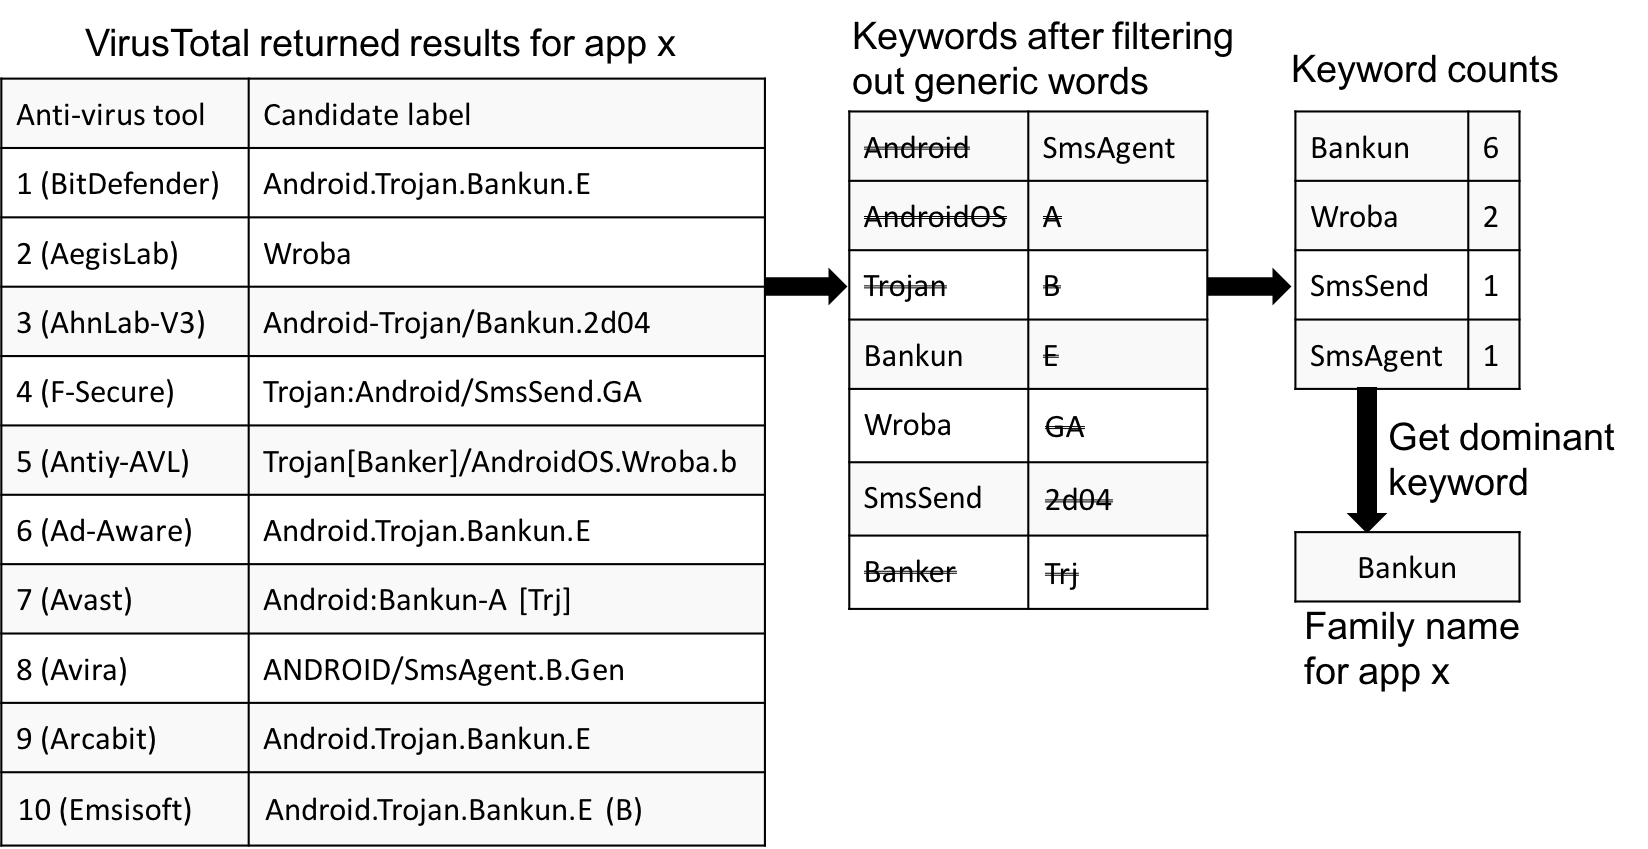
\includegraphics[width=3.8in]{fig/dominant.png}
\caption{Dominant keyword algorithm: identifying the malware family name of app $x$ from VirusTotal scan results of app $x$. Not all AV tools are listed here to save space.}
 \label{fig:dominant}
\end{figure}

This process is very similar to \emph{AVclass}~\cite{sebastian2016avclass},
although we developed the approach independently without the knowledge of
the AVclass work.
% \xo{Check later}
% The main difference is that not all samples can be labeled with concrete malware family name.
% We have seen lots of cases that: samples either not have sufficiently high AV labels or have
% sufficiently high AV labels but no dominant keyword.
An example is illustrated in Figure~\ref{fig:dominant}, in which 
(1) We show VirusTotal result for an app (to save space
we show only 10 anti-virus products' candidate labels for this app)
(2) We extract the keywords from each of the result, and get a list of keywords such as
\emph{Android}, \emph{AndroidOS}, \emph{Bankum}, \emph{Wroba}, \etc
We filter out the generic keywords such as \emph{Android}, \emph{AndroidOS}, and \emph{Trojan}.
(3) We count the remaining keywords, and get \emph{Bankun} as the dominant keyword, 
which is thus considered the family name.
In particular, \emph{Bankun} appeared 6 times,
which is greater than 50\% of the total results ($6 > 10 \times 50\%$), and
more than twice of the count of the second dominant keyword \emph{Wroba} ($6 > 2 \times 2$).

Out of the 52,520 apps obtained from step (1), we have \samsize samples left after step (2).
The rest are filtered out due to inconsistent family labels.
%27,861 apps are labeled as malware by at least 50\% of AV products but
%there is no consistent family name based on the criteria above.

\subsubsection{Discussion}

%We started with around 1.47 million raw app samples, and the above process returns
%only \samsize samples with reliable family names.
%Note that our goal is to present insights into the current landscape of Android malware. The more 
Our goal is to provide a reliable ground truth dataset that presents insights into the up-to-date landscape of Android malware. The more 
anti-virus companies agree with the labeling for a malware sample, the more popular such family is 
and thus it is a more important representative to serve our purpose.
%Since the objective of this work is to provide a reliable ground truth dataset, 
We leave as future work to analyze those apps that as of now have no dominant family names. 
%We expect
%some of them will start to have dominant names when AV products improve. For those that remain unresolved 
%the only option is manual analysis to assign a (possibly new) family label. Manual analysis
%techniques introduced in section~\ref{sec:manual} can be applied.

% For the app samples that are filtered out by the dominant keyword algorithm, significantly more manual 
% work would be needed to identify the correct family label for the samples; the manual analysis
% process we explain later could be applied for this purpose.

%  would be
% interesting to study as well, the ones we collected  with dominant labels from anti-virus companies
% are more important to study
% the more popular such family is; and thus we argue that the 30,000 samples we collect are more 
% important representative to serve our purpose.


% However, we remind the reader that our goal is to present the landscape of malware, and thus the above 
% is not a big issue to our study due to the following: 
\subsection{Identifying Malware Behavior Groups -- Varieties}

%In order to prepare a reliable ground truth, we perform multiple analyses (as discussed below) with help
%of a few assistance tools. The assistance tools include clustering analysis tool and reverse engineering tool.
It will not be feasible to perform deep manual analysis on each of the sample apps due to the large 
number of samples.
%to understand their behaviors. But that will be prohibitively expensive in terms of human labor.
%We may manually handle hundreds of apps, but to analyze in the scale of few thousands or even more is not manageable. 
How to reduce the amount of labor while maintaining the reliability of the result is a big challenge.
While one may think that samples under the same family name should have similar behaviors, 
%we can simply choose few samples from each malware family and complete the manual study.
the reality is that the family name of a malware typically 
%(\eg an output of dominant keyword algorithm) 
does not carry much semantic information. Anti-virus scanners name a malware
with different and often inconsistent conventions~\cite{hurier2016lack}. Sometimes, a scanner names a malware after
the malware writer Id; Other times the assigned family name is to highlight the main activities of the app (\eg \fn{FakePlayer})
or main goal of the app (\eg \fn{BankBot}), and so on. A malware app can achieve a goal through
different schemes. % and hence have different behaviors.
Thus the samples of a malware family can be very different in terms of their behaviors. 
Hence, we have to categorize the family members into semantically different groups which we call {\it varieties}. 
During our study, we observed that many families have more than one varieties.

This motivates us to apply a clustering analysis for a malware family to categorize
the samples into different varieties.
% and then perform manual analysis for just a few apps randomly selected from each variety.
% \vspace{-.1in}
% \subsubsection{Extracting varieties from a malware family}
% \label{sec:data:ground:variety}
% The large size of a malware family is a challenge for manual inspection.
% Another challenge is to identify the malicious part of the app. In particular,
% A malware app could be standalone in nature or repackaged on top of a benign app; so to extract
% only the malicious part (malicious payload) is useful for analysis.
% In order to overcome the aforementioned two challenges,
For a given family malware apps, we use a Android malware clustering analysis tool~\cite{li17:clustering}
to further categorize the labeled malicious apps into multiple varieties~(Figure~\ref{fig:methodpipe}).
Each variety of apps reported by the clustering algorithm contains a unique version of 
malicious payload.
Then, we only need to study a few representatives of each variety (not all apps therein)
in the later manual analysis phase. This makes the whole manual analysis process scale. Details of the
clustering algorithm can be found in our technical report~\cite{li17:clustering}.

% The design of our clustering analysis tool is inspired by the differential-commonality
% analysis principle used in MassVet~\cite{chen2015finding}, which is a proprietary tool for app vetting.
% The main idea is as follows: 
% if we see that many apps share a chunk of code that is not a well known library, 
% then it is likely that the shared code is a malicious payload and these apps belong to the same malware variety.
% %In other words, it is unlikely that many apps would happen to share a code chunk merely due to coincidence.
% %previously wrote assumption: Between two apps in a variety, the shared payload size is more likely to be bigger than shared random code sequence.

% We use the fuzzy-hashing fingerprint scheme, which has been shown to be
% successful in malware clustering analysis~\cite{li2015experimental}.
% We map the byte sequence of
% each app to a similarity-preserving fingerprint ($fp$) in the form of a bit vector. 
% The more similar two apps' fingerprints are, the bigger their shared code chunk is, and vice versa. 
% % Let us represent the fingerprint ($fp$) of app $x$ as $fp_x$. 
% % If the hamming distance between $fp_x$ and $fp_y$ is less than
% % that between $fp_x$ and $fp_z$, then we can infer that bigger chunk of code sequence is
% % common between app $x$ and app $y$ compared to that between app $x$ and app $z$.
% % hence app $x$ and $y$ are more likely to have similar behavior.
% Using fuzzy hash finger prints, we build a white-list of libraries which are commonly used by Android apps.
% Then, we discard such library packages from all the apps under the study.
% We then compute the fingerprints of all the pair-wise commonalities between apps as 
% candidate malicious payloads. A hierarchical agglomerative clustering algorithm is applied
% to the candidate payloads to identify large clusters, which often indicate a number of 
% input apps sharing the same code sequence. Apps involved in such a cluster are then output 
% as a variety. The process iterates and in the end a family is categorized into one or more 
% varieties.
% % Now the challenge is how we discover the pairwise shared code block while the 
% % number of apps is large, and also how to determine the similarity/dissimilarity 
% % among the pairwise shared code blocks. To address the above, 
% % Using fuzzy hashing 
% We observe that the above process may not always find clusters accurately. % For instance, if many apps in 
% % two varieties A and B have significant commonality (\ie payload of A and payload of B share 
% % a big code chunk), then our cluster analysis might merge these two varieties into one cluster 
% % C and outputs only variety C, which is the common intersection between A's payload and B's payload.
% The accuracy of clustering can be improved through corrective feedback from manual analysis 
% (ref. Fig.~\ref{fig:methodpipe}) as discussed later.  

%\begin{comment}
%\ptitle{Clustering Algorithm (CA)}
%In particular, the input to clustering algorithm (CA) is fingerprints of a family of apps, and the output is the varieties 
%(as wells as the corresponding payloads) present in the family. The CA consists of the following steps.
%
%1. For each pair of $fp$ (say $fp_i$ and $fp_j$), compute the commonality (denoted by $fp_{ij}$).
%Note that this gives us O($n^2$) items called {\it pairwise commonalities}.
%
%2. With a similarity preserving distance function defined (\eg hamming distance as in Yuping2015), use a 
%clustering technique (\eg hierarchical agglomerative clustering) to categorize
%the {\it pairwise commonalities}. This step gives us a group of clusters whereas an app is associated with multiple clusters.
%
%3. Starting from the biggest cluster found above, we assign the membership of each $fp_i$.
%Once an $fp_i$ is already assigned, it cannot be assigned to another cluster.
%We continue this process until we are done with all clusters (\ie processing the smallest cluster at the end).
%Note that an app is associated with only one cluster after this step. So, this step leaves us with a set of {\it active} clusters.
%
%4. For each {\it active} cluster, extract the commonality of the member apps,
%which gives us the payload. Each {\it active} cluster also corresponds to a variety of apps. 
%
%Let us take an example to illustrate the clustering analysis.
%\end{comment}

%The rationale behind this algorithm is that 
%(1) If different app are sharing same code and
%the code are not belonging to white-listed third party libraries then it is malicious payload;
%(2) If the same malware family's malicious apps/payloads are dramatically different from each
%other, than it belongs to different varieties of this malware family.
%After the tool run for each malware family, we can get which malware family is repackaged,
%what are the payload part, and how many varieties exist in this family.
%Because with in each variety of a malware family, the malicious code are very similar, so
%we can choose few of them to represent this whole variety, which dramatically decreased
%the labor force of analyzing large number of apps.

%For the labeled malware families, it is possible that 
%samples from the same family contain different varieties of malicious payloads.
%To discover such varieties within a malware family, we use a home-brewed Android-based clustering tool. In particular,
%our tool extracts the payload (if the sample is a repackaged app) and then cluster (payload-sharing-based clustering) 
%the samples based on the overall similarity of the payload's bytecode sequence.
%The technical details of our clustering tool will be published as a tech report
%together with this paper.
%Discovering different varieties (if present) within a malware family not only helps us understand how active the malware family is
%but also lets us identify the evolution trace of such a family.
%Moreover, discovering varieties help us organize our study in identifying new behaviors (\ie not have been reported before) of malware.
%At this phase, if two malware sample have more than 80\% similarity, we consider they belong to one variety.

\vspace{-.1in}
\subsection{Manual Analysis}
\label{sec:manual}
We manually analyze each variety of malware samples. If a variety contains more than three samples, 
we randomly select three of them for manual analysis. Otherwise, we analyze all samples in 
the variety. Through a systematic study of the samples, we generate a detailed report 
on the malware variety's behavior.

\subsubsection{Challenges}
\vspace{-.1in}
\begin{enumerate}[label=\alph*)]
\item Manually analyzing a malware sample warrants a systematic strategy; 
without a strategy it is nearly impossible
 to understand the comprehensive picture of a malware's behaviors.
\item Anti-analysis/obfuscation techniques are commonly used in Android apps as well as in malware payloads,
which has an adverse impact both on static analysis tools and to the analyst who wants 
to understand the semantics of the given app. 
\item The malware app itself may not always contain the full information. Many components could be
fetched from a remote server while the malware runs on the infected device, and those servers
may have already been taken down after the malware app was identified. Thus it may be impossible for 
us to obtain those missing parts for analysis.
\end{enumerate}

\subsubsection{Assistance Tools}

When manually analyzing malware apps, we leverage available tools and 
frameworks wherever they are relevant and helpful. 
A static analysis tool with capability of 
collecting apk information and performing
reachability analysis can help the analyzer quickly prioritize the analysis process.
An appropriate tool can help obtain the trace to critical APIs.
For instance, when analyzing renamed obfuscated apps, we cannot easily guess the semantics
of the classes and methods. In that case, we should locate the critical API calls (\eg openConnection,
sendTextMessage) and perform reachability analysis to understand from which component this API
gets invoked, and track the call chain to get a more clear picture of what
the app is doing.
To serve this purpose, we leverage Amandroid~\cite{wei2014amandroid} which is a publicly 
available\footnote{Tool website: \url{http://pag.arguslab.org/argus-saf}}
comprehensive static analysis framework for analyzing Android apps.

In addition, an IDE-like editor that provides functionality of 
class hierarchy resolution, def-use chain building, method invocation tracing in
the decompiled IR (intermediate representation) is also to the human analysts to
understand the code flow. We built such an analysis tool for this 
purpose\footnote{Tool website: \url{http://pag.arguslab.org/argus-cit}}.

% use a homebrew tool which can take the decompiled
% apk from \emph{Amandroid} and then can support IDE style editing on it.

An Android app development environment is also important for manual analysis. 
An analyst may need to ``re-implement'' certain parts of the malware to test 
the real functionality, or to get the runtime value of certain variables.
For instance, many malware apps encrypt the string constant and the malicious 
payloads to avoid detection. 
When analyzing such a malware, we first identify the decryption routine, extract 
and load it in a separate app, and then provide the 
encrypted content to get the plaintext information.

\subsubsection{The Overall Strategy of Manual Analysis}

With the help from the aforementioned assistance tools, 
we performed manual analysis of 405 Android 
malware samples representing \versize varieties.
Here we present a systematic way of how to manually analyze Android malware, which 
serves as a guideline for other people who want to reproduce our analysis results, 
or to analyze other Android malware apps.

\ptitle{Identifying Malicious Components}
An Android app is organized as a collection of components. To understand the behavior of a given
malware sample we have to identify which components belong to the malware payload,
or whether the whole app is a standalone malware.
As the clustering analysis (CA) tool~\cite{li17:clustering} we use is imperfect, 
the payload it outputs for each variety
could be the full payload or a partial payload.
For the latter case, we need more effort to identify the full payload.
We get help from the following observations: 
(1) Since a component is the basic functional block for an Android app, we can expect that the full component is
likely to belong to the payload, if a few of the component's methods
or reachable methods appear in the CA-extracted payload;
(2) In most cases, the package name is a good indicator; if some of a package's classes appear in 
the CA-extracted malicious payload, then the whole package is very likely to belong to the payload.
Malware writers could also instrument the benign part of the repackaged malware
to initialize the payload, so we should also search for any use of payload package names inside
the benign components. This will enrich our understanding of the activation strategy for this malware.
%if the payload size is much smaller than the whole app.
%However, if the payload size is close to the app size, it is hard to say if it is repackaged or
%standalone because it could be repackaged on top of a very simple app, or
%there can be only minor difference between samples inside this standalone malware 
%variety.
%In that case, we need to study the whole app to understand whether all the components are
%contributing to the malware behavior, or it still has a benign part.

\ptitle{Prioritizing Component Analysis}

We should not start the analysis from a random component as that will not put the analysis in a meaningful context. 
% Unless we get the right context, the analyzer might waste much of her time.
After obtaining the malicious components using the CA tool,
we follow a triaging scheme, and analyze the components in the following sequence:

\begin{enumerate}[label=\alph*)]

\item Event handlers:
Event handlers mostly serve as the entry points in an Android app.
More specifically,
the main Activity and 
the BroadcastReceiver receiving \mbox{``android.intent.action.BOOT_COMPLETED''} event \linebreak
(\mbox{BootReceiver})
is the initializer, which can be used to start the core component (\eg monitor service) of the malware,
so it should be analyzed first.
Other event handlers are mainly related to monitoring user information and
the environment of infected device.
They also can be considered as entry points of certain malware.
Take as example a BroadcastReceiver which receives
``android.provider.Telephony.SMS_RECEIVED''. This component is used
to listen to any new incoming SMS message for this device. When we analyze such a component,
we should check how it handles the message, whether it performs some operation related to the device inbox,
if it matches the incoming message phone number with some list
(\eg bank phone numbers, vendor phone numbers, \etc), and aborts the SMS using
abortBroadcast() method call.

\item The services that are started by initializers normally contain the main logic of the
malware (monitor service); thus they need to be analyzed as soon as possible.
It is the core component for most malware, which the malware will try
to keep running as long as possible. It is common to see that many entry point components
or scheduled tasks will start such service. 
The monitor service normally is used to fetch and reply to commands from
a command and control server. It is also common to schedule some TimerTask or BroadcastReceiver
to constantly check the internet connectivity, whether an anti-virus product is running,
whether itself is still alive, and so on.

\item All remaining components.
The purpose of those components vary. The guideline is to
start from such a component and
trace all the reachable code to understand: 
(i) what role the component plays, 
(ii) which other components this component communicates with,
(iii) which BroadcastReceiver this component registers, 
(iv) whether this component starts some thread or AsyncTask and what is the purpose.
\end{enumerate}

%BroadcastReceiver could be dynamically registered and avoid
%appearing in the Manifest file. This could increase the analysis complexity.

%{\bf Component Analysis.}
%After we pick one component to start analysis, we trace the methods from such a component to all
%the reachable code to understand: 
%(1) what role the component plays, 
%(2) which other components this component communicates with,
%(3) which BroadcastReceiver this component is registering, 
%(4) whether this component starts some thread or AsyncTask and what is the purpose.
%Normally, the MainActivity  or BootReceiver
%plays the role of the initializer for the malware.
%Those components will be used to start the monitor service, which is the most important component
%for most of the malware. It is also possible to register some BroadcastReceivers dynamically
%to listen to events like ``android.intent.action.PHONE_STATE'',
%``android.provider.Telephony.SMS_RECEIVED'',
%``android.net.conn.CONNECTIVITY_CHANGE'', which can avoid those BroadcastReceiver
%to appear in the Manifest file, thus increasing the analysis complexity.
%%From initializer we find what the monitor Service is.
%The monitor Service is the core component for most malware, which the malware will try
%to keep running as long as possible. It is normally used to fetch and reply command from
%a command and control server. It is also common to schedule some TimerTask or BroadcastReceiver
%to constantly check the internet connectivity, whether anti-virus product is running,
%whether the monitor Service is still alive, \etc 
%When analyzing those manifest-defined or dynamically registered BroadcastReceivers, we first
%check what kind of events it is handling. Take a BroadcastReceiver which receives
%``android.provider.Telephony.SMS_RECEIVED'' as an example. This component is used
%to listen to any new incoming SMS message for this device. When we analyze such a component,
%we should check how it handles the message, whether it performs some operation related to the device inbox,
%if it matches the incoming message phone number with some list, and aborts the SMS using
%abortBroadcast() method call.

\pagebreak

\ptitle{Building the Behavior Report}
After we analyze all the relevant components, we generate a report that
includes an inter-component graph where a node represents a component 
(present in the malicious payload) or a worker thread loaded by such a component, and an edge represents 
the communication/interaction between two nodes. 
The graph also illustrates behavior description for each node and edge, such as
the activation method, communication message, C\&C commands, \etc
%the components, activation method for each of them, how/what
%they communicate, what functionality they have, \etc
This gives us a comprehensive picture of the malware on top of which  
we can understand its richer behavior, \eg what is the monetizing method,
how it maintains the persistence, its main goal, and so on.
% We also summarize all the behaviors among all our malware families to generate a 
% comprehensive table as discussed later.
The behavior report including the inter-component graph for each malware variety is 
available at the \amd.

\subsubsection{Handling Anti-analysis/Obfuscation}

\begin{enumerate}[label=\alph*)]

\item Renaming: Class name, method name and field name are important hints for understanding
the malware's purpose. Renaming them to meaningless words makes manual analysis difficult.
We can get help from static analysis tools to perform a reachability analysis to see all the
reachable methods from a given component. This can help us locate the interesting APIs 
(as the system API names cannot be renamed). We follow the call trace to understand 
how an API gets invoked and
how the calling parameters are prepared. 

\item String encryption: Oftentimes, we understand the malware behavior based on the strings used
in the code, like URL, C\&C command, class names, phone number, \etc
If those strings are encrypted, it is very difficult to understand the semantics of those actions.
To address this issue, we analyze the malware code to figure out the decryption routine and key.
We then re-implement it in a separate app to decrypt the strings.
\item Dynamic loading: Malware may hide its functionality in a separate apk/dex file and load it
dynamically at runtime. Even worse, apk/dex file may be encrypted. To handle such cases, we first
retrieve the decryption routine to decrypt the apk/dex file. For either case we decompile the code to study it 
as a regular app, which adds to our understanding of the malware.
\item Native payload: Most Android static analysis tools do not handle native code. Thus malware writers
like to put some core function or data in the native payload. For us to understand how the native
payload works, we use standard binary reverse-engineering tools including IDA~\cite{ida} and hexdump~\cite{hexdump}.
\end{enumerate}

\subsubsection{Handling Missing Contents}

Sometimes, we may not be able to obtain the full payload of the malware,
but we still have ways to maximize our understanding.
The basic idea is to understand how the malware leverages the missing content.
For instance, if we observe that the malware downloads an apk file, we could see
whether this malware sends an installation request for this apk or it uses \emph{DexClassLoader}
to load some new classes. In the first case, we could check the description of the installation
request (which will show up on the screen to the device user) to understand the purpose of such
action. For example, this description may say ``Crucial update found for xxx.'' Then we know it 
is misleading the user to install a malware.
In the second case, we know this malware is dynamically loading some code; we should expect to see
multiple java reflection calls to such code, and from those reflection calls we could infer what
role it plays.

% \subsubsection{Corrective Feedback}

% We experienced that the manual analysis can provide a corrective feedback to the clustering analysis. 
% We understand that clustering analysis may not be perfect and some of the results may have room for 
% better accuracy. 
% As an example, the human analyzer can come to know a new package inside the app that is a 3rd party library but it is not yet 
% present in the white-list of library packages maintained by the cluster analysis tool.
% We use feedback from the manual analysis to make cluster results better. There are two possible scenarios: 
% (i) If after picking a random sample $x$ from a variety, 
% we see that its behavior is very different from other apps in the same variety, then we classify $x$ as a separate variety. 
% We have not yet encountered such case in our experience. (ii) If the random samples from a variety $i_1$ seems to be very similar to 
% random samples in another variety $i_2$, we merge $i_1$ and $i_2$ into a single variety. This scenario did occur in our experience.
% %Note that in Section~\ref{sec:data:ground:variety}, we discuss the reason for possibility of such issues from the cluster analysis tool.

\subsubsection{Discussion}

One may wonder what is the benefit of our study given the fact that
after a malware family is discovered, anti-virus companies usually publish 
a report/bulletin on a sample app from that family. 
In fact, for each family under our study (71 in total), we did find such 
reports on the web. % Given the above, someone may 
% doubt on the utility of our study. We remind the reader that
However, such reports usually only highlight the security breaches and 
main activities of the malware family and do not describe the malware behaviors in details.
This is not sufficient for malware research. In addition, those reports do not provide 
the varieties for each family and the different malware behaviors from those varieties. 
% Another limitation of such reports is that each of them focuses on a particular malware family, and 
% does not give us the comprehensive malware landscape unlike our study.

%No clustering tool is perfect, \ie they all occasionally make mistakes. 
%For our case, the samples having different
%bytecode structure may not necessarily mean they belong to different variety.
%So, in the manual verification phase, we choose two to three samples from
%each variety (obtained in the above Malware Clustering phase) to manually inspect their behaviors,
%take detailed notes, and analytically compare the behaviors. Finally, if deemed necessary, we merge mis-clustered varieties.
%Due to the extensive use of obfuscation techniques in malware
%samples, the manual analysis process poses many challenges.
%For each of the obfuscated samples under analysis, we build a deobfuscation
%scheme to decrypt the encrypted strings and payload files, which finally make the analysis
%possible. In the end, we obtained \versize varieties of \fsize from \samsize samples.

%%% Local Variables: 
%%% mode: latex
%%% TeX-master: "paper"
%%% End: 
